
In this appendix we detail the methods used to create the random two-dimensional tri-coordinated lattices used in Chapters \ref{chap:chern_intro} and \ref{chap:local_markers} to create the amorphous analogue of the QWZ model, and in Chapter \ref{chap:amorphous_kitaev} to construct the amorphous Kitaev model. This is done using the Voronoi partition \cite{voronoi_nouvelles_1908}, which well-known in the physics community as the method used to produce a Wigner-Seitz unit cell \cite{wigner_contstruction_1933}. The method allows one -- given a set of $n$ points -- to partition the plane into a set of $n$ regions. Each of these regions contains the area of the plane that is closer to a given point than any other, with the boundary between two regions always being perpendicular to the line connecting their two respective points. 

In practice, fast routines exist for constructing a Voronoi partition, we used a built-in function from the python package /\texttt{scipy}, namely \texttt{scipy.spatial.Voronoi}, which uses the quickhull algorithm \cite{barber_quickhull_1996}. The only complication comes from working in periodic boundary conditions, since the algorithm is designed for open boundary systems. This is straightforwardly solved by tiling the system before computing the Voronoi partition. Then, once a Voronoi diagram has been constructed, we restrict back to the unit square, identifying the unit-separated vertices that should equivalent under periodic boundaries. An example is shown in Fig.~\ref{fig:voronoi}. 

A Voronoi lattice can now be extracted from the Voronoi partition by assigning an edge to the boundary between every pair of cells, and a vertex to the points at which three cells meet. This lattice will always be tri-coordinated, provided that none of the original seed points lie at the corners of a regular $m$-sided polygon, since this would lead to the formation of an $m$-coordinated vertex at the centre of that polygon in the Voronoi lattice. 

\begin{figure}
    \centering
    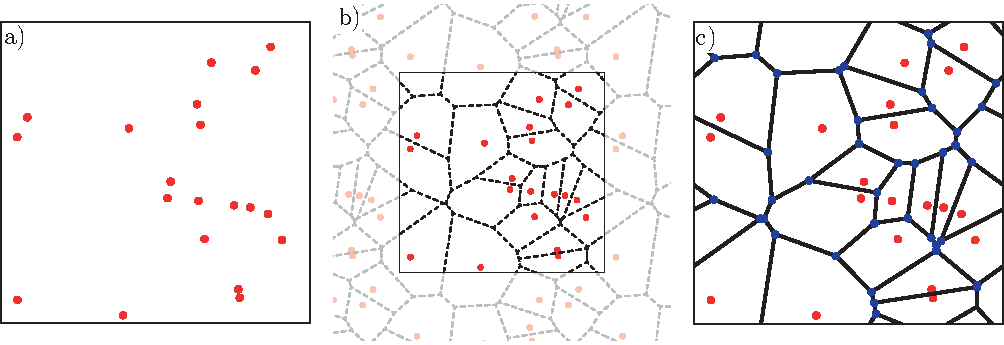
\includegraphics{appendices/figures/voronoi.pdf}
    \caption [A Voronoi partition calculated in periodic boundaries.]{
        An example Voronoi partition calculated for a set of 20 points on the unit square in periodic boundaries.
        \textbf{(a)}~The initial set of 20 points, sampled uniformly on the square.
        \textbf{(b)}~In order to construct a partition consisted with periodic boundary conditions, the initial set of points is tiled, creating eight copies around the central region. Now a Voronoi diagram is calculated for this extended system, corresponding to the dashed lines. 
        \textbf{(c)}~We restrict back to the unit square, identifying vertices that should be equivalent, resulting in a final, periodic, Voronoi partition. A Voronoi lattice is now identified by the edges and blue vertices, each of which sits at the point of intersection of three Voronoi cells. 
    }
    \label{fig:voronoi}
\end{figure}


\section{Lloyd's Algorithm}

Typically, lattices generated via Voronoi partition do not resemble real amorphous materials. This is because, when a set of seed points are arranged roughly equidistant from a central point, the Voronoi partition will place a cluster of vertices extremely close to one another at that point. An example is seen in the green-shaded area in Fig.~\ref{fig:lloyd}a. In general, physical materials usually have some condition that prevents vertices (or atoms) from becoming extremely close to one another. Thus, in order to generate more physically applicable random lattices, we use Lloyds algorithm to approximately evenly space the vertices in a lattice. The algorithm is straightforward, consisting of three steps which are repeated:
\begin{enumerate}
    \item Given a Voronoi partition, a new set of seed points are generated for each cell, defined as the centre of mass of each cell.
    \item The original seed points are then moved to these new centre-of-mass points.
    \item Now the Voronoi lattice is recalculated using the new points, producing a new Voronoi diagram that is slightly more regular than the original.
\end{enumerate}
An example of one step in this process is shown in fig.~\ref{fig:lloyd}. 
\begin{figure}
    \centering
    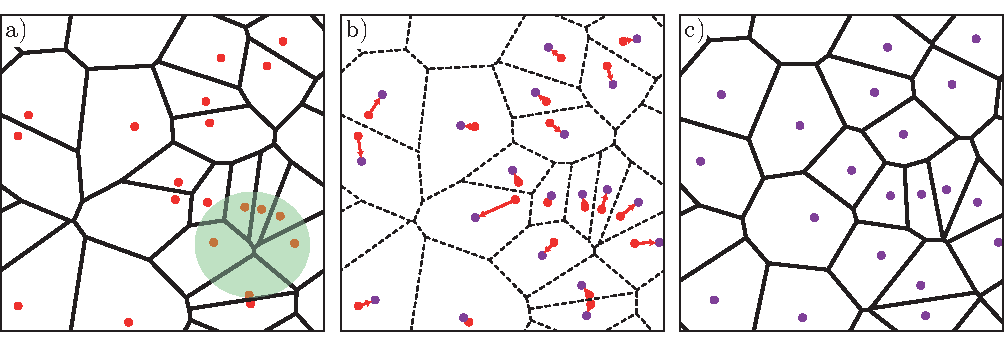
\includegraphics[]{appendices/figures/lloyd.pdf}
    \caption [One step of Lloyd's algorithm.]{
        One step of Lloyd's algorithm is shown.
        \textbf{(a)}~The initial Voronoi lattice is shown, with initial seed points shown in red. The green highlighted area shows a series of points that would be unphysical in a physics model, since they are extremely close to one another.  
        \textbf{(b)}~New seed points are calculated for each cell, positioned at the centre of mass of the cell. The seed points are then moved to these new positions. 
        \textbf{(c)}~The Voronoi lattice is recalculated, producing a new, more evenly spaced lattice. 
    }
    \label{fig:lloyd}
\end{figure}

With each successive application of this algorithm, the lattice will become increasingly regular. In Fig.~\ref{fig:lloyd_successive} we show the result of applying 5, 50 and 150 iterations of this process to the Voronoi partition generated in Fig.~\ref{fig:voronoi}. 

\begin{figure}
    \centering
    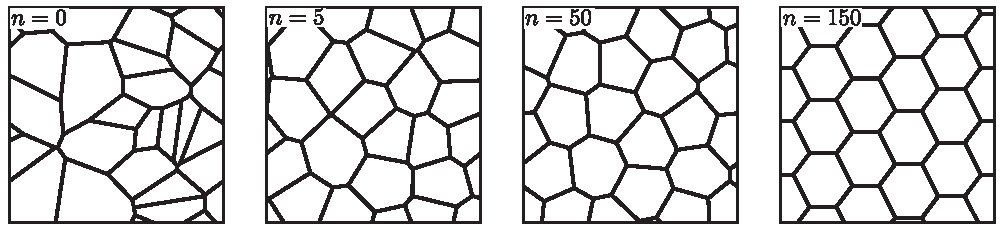
\includegraphics[]{appendices/figures/lloyd_successive.pdf}
    \caption[The effect of successive iterations of Lloyd's algorithm on a Voronoi lattice.] {
        Four Voronoi lattices are shown, each corresponding to performing $n$-steps of Lloyd's algorithm to the Voronoi lattice generated in Fig.~\ref{fig:voronoi}. After around 150 steps, successive iterations of the algorithm produce no changes.
    }
    \label{fig:lloyd_successive}
\end{figure}


